\documentclass[aspectratio=169, 9pt]{beamer}\usepackage[]{graphicx}\usepackage[]{color}
% maxwidth is the original width if it is less than linewidth
% otherwise use linewidth (to make sure the graphics do not exceed the margin)
\makeatletter
\def\maxwidth{ %
  \ifdim\Gin@nat@width>\linewidth
    \linewidth
  \else
    \Gin@nat@width
  \fi
}
\makeatother

\definecolor{fgcolor}{rgb}{0.345, 0.345, 0.345}
\newcommand{\hlnum}[1]{\textcolor[rgb]{0.686,0.059,0.569}{#1}}%
\newcommand{\hlstr}[1]{\textcolor[rgb]{0.192,0.494,0.8}{#1}}%
\newcommand{\hlcom}[1]{\textcolor[rgb]{0.678,0.584,0.686}{\textit{#1}}}%
\newcommand{\hlopt}[1]{\textcolor[rgb]{0,0,0}{#1}}%
\newcommand{\hlstd}[1]{\textcolor[rgb]{0.345,0.345,0.345}{#1}}%
\newcommand{\hlkwa}[1]{\textcolor[rgb]{0.161,0.373,0.58}{\textbf{#1}}}%
\newcommand{\hlkwb}[1]{\textcolor[rgb]{0.69,0.353,0.396}{#1}}%
\newcommand{\hlkwc}[1]{\textcolor[rgb]{0.333,0.667,0.333}{#1}}%
\newcommand{\hlkwd}[1]{\textcolor[rgb]{0.737,0.353,0.396}{\textbf{#1}}}%
\let\hlipl\hlkwb

\usepackage{framed}
\makeatletter
\newenvironment{kframe}{%
 \def\at@end@of@kframe{}%
 \ifinner\ifhmode%
  \def\at@end@of@kframe{\end{minipage}}%
  \begin{minipage}{\columnwidth}%
 \fi\fi%
 \def\FrameCommand##1{\hskip\@totalleftmargin \hskip-\fboxsep
 \colorbox{shadecolor}{##1}\hskip-\fboxsep
     % There is no \\@totalrightmargin, so:
     \hskip-\linewidth \hskip-\@totalleftmargin \hskip\columnwidth}%
 \MakeFramed {\advance\hsize-\width
   \@totalleftmargin\z@ \linewidth\hsize
   \@setminipage}}%
 {\par\unskip\endMakeFramed%
 \at@end@of@kframe}
\makeatother

\definecolor{shadecolor}{rgb}{.97, .97, .97}
\definecolor{messagecolor}{rgb}{0, 0, 0}
\definecolor{warningcolor}{rgb}{1, 0, 1}
\definecolor{errorcolor}{rgb}{1, 0, 0}
\newenvironment{knitrout}{}{} % an empty environment to be redefined in TeX

\usepackage{alltt}

% \transdissolve[duration=0.2] % Only works with Adobe Acrobat

% \mode<handout>

% Some important packages
\usepackage{epstopdf}
\hypersetup{colorlinks=false, allcolors=purple}
\usepackage{booktabs}
\linespread{1.3}
\usepackage{tabularx}
\usepackage{makecell} % For makecell within tables
\usepackage{geometry}
\usepackage{algorithm2e}
\usepackage{amsmath, amssymb}
% Mathematical functions
% DELETED!
\renewcommand{\Pr}[1]{{\mathbb{P}\left(#1\right) }}
% DELETED!
% DELETED!
% DELETED!
% DELETED!
% DELETED!

% DELETED!
\newcommand{\sufstats}[1]{s\left(#1\right)}
\renewcommand{\exp}[1]{\mbox{exp}\left\{#1\right\}}
\newcommand{\transpose}[1]{{#1}^\mathbf{t}}

% Objects
% DELETED!
% DELETED!
\newcommand{\Graph}{\mathbf{G}}
\newcommand{\graph}{\mathbf{g}}
\newcommand{\GRAPH}{\mathcal{G}}
\newcommand{\Adjmat}{Y}
\newcommand{\adjmat}{y}
\newcommand{\ADJMAT}{\mathcal{Y}}

\newcommand{\INDEPVAR}{\mathcal{X}}
\newcommand{\Indepvar}{X}
\newcommand{\indepvar}{x}

\newcommand{\normconst}{\kappa\left(\params, \Indepvar\right)}

\graphicspath{{./figures/}{.}{./terms/}}


%% NEED THIS FOR CANCY TEX
\usepackage{pstricks}

% Colors
\definecolor{USCCardinal}{HTML}{990000} % 153 0 0 in RGB
\definecolor{USCGold}{HTML}{FFCC00}
\definecolor{USCGray}{HTML}{CCCCCC}

% To use the function \sout
\usepackage{ulem}
\usepackage{tabularx, booktabs}

% \bibliography{bibliography.bib}

\def\ergmito{ERGM\textit{ito}}
\def\ergmitos{\ergmito{}\textit{s}}
% Mathematical functions
\newcommand{\isone}[1]{{\boldsymbol{1}\left( #1 \right)}}
\renewcommand{\Pr}[1]{{\mathbb{P}\left(#1\right) }}
\newcommand{\f}[1]{{f\left(#1\right) }}
\newcommand{\Prcond}[2]{{\mathbb{P}\left(#1\vphantom{#2}\;\right|\left.\vphantom{#1}#2\right)}}
\newcommand{\fcond}[2]{{f\left(#1|#2\right) }}
\newcommand{\Expected}[1]{{\mathbb{E}\left\{#1\right\}}}
\newcommand{\ExpectedCond}[2]{{\mathbb{E}\left\{#1\vphantom{#2}\right|\left.\vphantom{#1}#2\right\}}}
\renewcommand{\exp}[1]{\mbox{exp}\left\{#1\right\}}

\newcommand{\Likelihood}[2]{\text{L}\left(#1 \left|\vphantom{#1}#2\right.\right)}

% Mathematical Annotation -------------------------------
% Modify this so that it matches the P01 convention overall

% Tree
\newcommand{\phylo}{\Lambda{}} % The actual tree
\newcommand{\aphylo}{D{}}      % The annotated phylogenetic tree
\newcommand{\aphyloObs}{\tilde \aphylo{}} % The observed annotated phylogenetic tree
\newcommand{\parent}[1]{\mathbf{p}\left(#1\right)}
\newcommand{\offspring}[1]{\mathbf{O}\left(#1\right)}
\newcommand{\nodes}{\mathcal{N}{}}
\newcommand{\edges}{\mathcal{E}{}}

\newcommand{\class}[1]{C_{#1}{}}

% Annotations
\newcommand{\Ann}{\mathbf{X}{}} % Matrix of "real" annotations
\newcommand{\ann}[1]{x_{#1}{}} % single element of "real" annotations
\newcommand{\constraints}{\mathcal{C}{}} % Taxon constraints

% Obs Annotations
\newcommand{\AnnObs}{\mathbf{Z}{}}%{Z{}} \mathbf{X}^{obs}{}
\newcommand{\annObs}[1]{z_{#1}{}}%{z{}}  x_{#1}^{obs

% Pred. Annotations
\newcommand{\AnnPred}{\hat X{}}
\newcommand{\annPred}[1]{\hat x_{#1}}

% Leaf nodes
\newcommand{\Leaf}{L{}}

% Shortest path
\newcommand{\Geodesic}{\text{T}{}}
\newcommand{\geodesic}{\tau{}}

\newcommand{\Params}{\Omega{}}
\newcommand{\params}{\omega{}}

% Parameters
\newcommand{\gain}{\mu_{01}{}}
\newcommand{\loss}{\mu_{10}{}}
\newcommand{\misszero}{\psi_{01}{}}
\newcommand{\missone}{\psi_{10}{}}
\newcommand{\proot}{\pi}


\usepackage[style=authoryear-comp]{biblatex}
\addbibresource{bibliography.bib}
% \renewcommand{\bibsection}{\subsubsection*{\bibname } }


% Styles
\usepackage{xcolor}
\usepackage{colortbl}
\definecolor{suffstat}{RGB}{10,159,0}
\definecolor{normconst}{RGB}{87,38,231}
\setbeamercolor{conclusions}{bg=usclightgray!60!white, fg=uscdarkgray}

% Noice!
\usetheme{usckeck}

\title[Stat. Comp. for Complex Systems]{Essays on Bioinformatics and
Social Network Analysis
\linebreak{\small Statistical and Computational Methods for
Complex Systems}}
\author[GGVY]{George G Vega Yon}
\institute[USC-PREVMED]{University of Southern California, Department of Preventive Medicine}
\date{January 28, 2020 }

% Some definitions
\def\cursection{\frame{\frametitle{Contents}\tableofcontents[current]}}
\newcommand{\ergmpkg}[0]{\texttt{ergm}}
\newcommand{\ergmitopkg}[0]{\texttt{ergmito}}
\newcommand{\aphylopkg}[0]{\texttt{aphylo}}
\graphicspath{{.}{fig/}}


% ------------------------------------------------------------------------------
% ------------------------------------------------------------------------------
% --------------------------- END OF PREAMBLE ----------------------------------
% ------------------------------------------------------------------------------
% ------------------------------------------------------------------------------
\setbeamertemplate{note page}[plain]
%\setbeameroption{show notes}
\usepackage{pgfpages}
% \setbeameroption{show notes on second screen}

\newcommand{\hlc}[2]{{\only<#1>{\cellcolor{gray!50} #2}}}
\newcommand{\nhlc}[2]{{\only<#1>{#2}}}
\IfFileExists{upquote.sty}{\usepackage{upquote}}{}
\begin{document}
% \SweaveOpts{concordance=TRUE}

% ------------------------------------------------------------------------------
\begin{frame}%[noframenumbering]
\maketitle
\end{frame}

% ------------------------------------------------------------------------------
\begin{frame}
\frametitle{What motivates my research}

\begin{center}
\large
\textcolor{usccardinal}{\bf Statistical and computational methods for\\ %
bioinformatics and social network analysis}
\end{center}

\begin{itemize}[<+->]
\item We live in a non-{\it IID} world.
\item In some times, the cannot understand a process unless we look at it as a whole.
\item There's a reason why we usually assume {\it IID}.
\item {\it Modern} (as of today) computational tools help us coping with that.
\end{itemize}
\end{frame}


\frame{\frametitle{Contents}\tableofcontents}

% ------------------------------------------------------------------------------
\section{Paper 2: Exponential Random Graph Models for Small Networks}
% \frame{\frametitle{Contents}\tableofcontents}

\begin{frame}[t]
\usebeamertemplate{section intro}{}{}
\textcolor{uscgold}{
\Large {\bf Exponential Random Graph Models for Small Networks} \vskip0.25em
\large \textit{Joint with}: Andrew Slaughter and Kayla de la Haye
}
\end{frame}

\begin{frame}
\frametitle{What are Exponential Random Graph Models}

Exponential Family Random Graph Models, aka \alert{ERGMs} are:\pause

\begin{itemize}[<+->]
\item Statistical models of (social) networks
\item In simple terms: statistical inference on what network patterns/structures/motifs
govern social networks
\begin{figure}
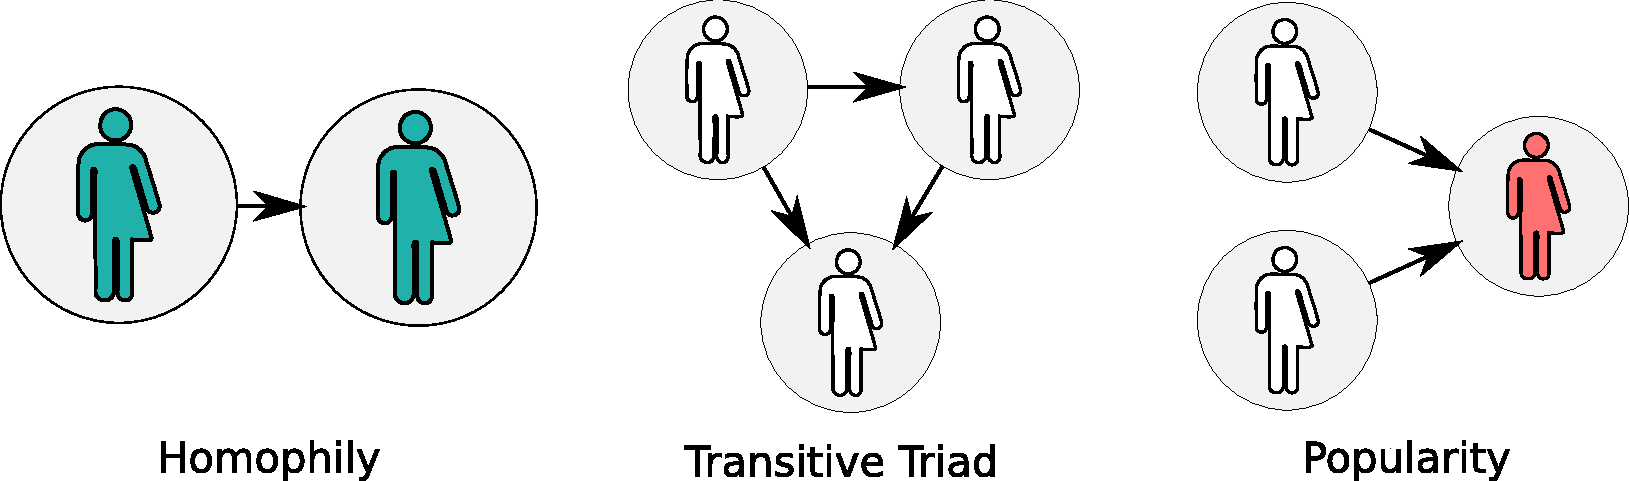
\includegraphics[width=.6\linewidth]{friendly-terms.pdf}
\end{figure}
\end{itemize}

\end{frame}

% ------------------------------------------------------------------------------
\begin{frame}[label=ergmeq]
\frametitle{ERGMs (cont'd)}
\begin{figure}
\centering
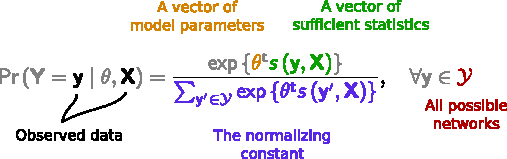
\includegraphics[width=.7\linewidth]{parts-of-ergm.pdf}
\end{figure}

\uncover<2->{The normalizing constant has $2^{n(n-1)}$ terms!}

% \vfill\hfill \hyperlink{ergmterms}{\beamergotobutton{more on terms}}
\end{frame}

% ------------------------------------------------------------------------------
\begin{frame}[label=ergmterms]

{\bf\color{suffstat} Sufficient statistics} have various forms

\def\fig1width{.45\linewidth}
\begin{figure}[tb]
\centering
\begin{tabular}{m{.2\linewidth}<\centering m{.4\linewidth}<\raggedright}
\toprule Representation & Description  \\ \midrule

\includegraphics[width=\fig1width]{ergm-terms/mutual.pdf} & Mutual Ties (Reciprocity)\linebreak[4]$\sum_{i\neq j}y_{ij}y_{ji}$  \\
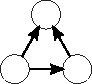
\includegraphics[width=\fig1width]{ergm-terms/ttriad.pdf} & Transitive Triad (Balance)\linebreak[4]$\sum_{i\neq j\neq k}y_{ij}y_{jk}y_{ik}$  \\

\includegraphics[width=\fig1width]{ergm-terms/homophily.pdf} & Homophily\linebreak[4]$\sum_{i\neq j}y_{ij}\mathbf{1}\left(x_i=x_j\right)$ \\
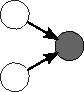
\includegraphics[width=\fig1width]{ergm-terms/nodeicov.pdf} & Covariate Effect for Incoming Ties\linebreak[4]$\sum_{i\neq j}y_{ij}x_j$ \\
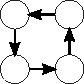
\includegraphics[width=\fig1width]{ergm-terms/fourcycle.pdf} & Four Cycle\linebreak[4]$\sum_{i\neq j \neq k \neq l}y_{ij}y_{jk}y_{kl}y_{li}$  \\
\bottomrule
\end{tabular}
\end{figure}

% \vfill\hfill \hyperlink{ergmeq}{\beamerreturnbutton{go back}}
\end{frame}

% -----------------------------------------------------------------------------
\begin{frame}[label=ergm-toyexample]

\begin{columns}[c]

\begin{column}[c]{.4\linewidth}

In this network\linebreak

\begin{knitrout}
\definecolor{shadecolor}{rgb}{0.969, 0.969, 0.969}\color{fgcolor}

{\centering 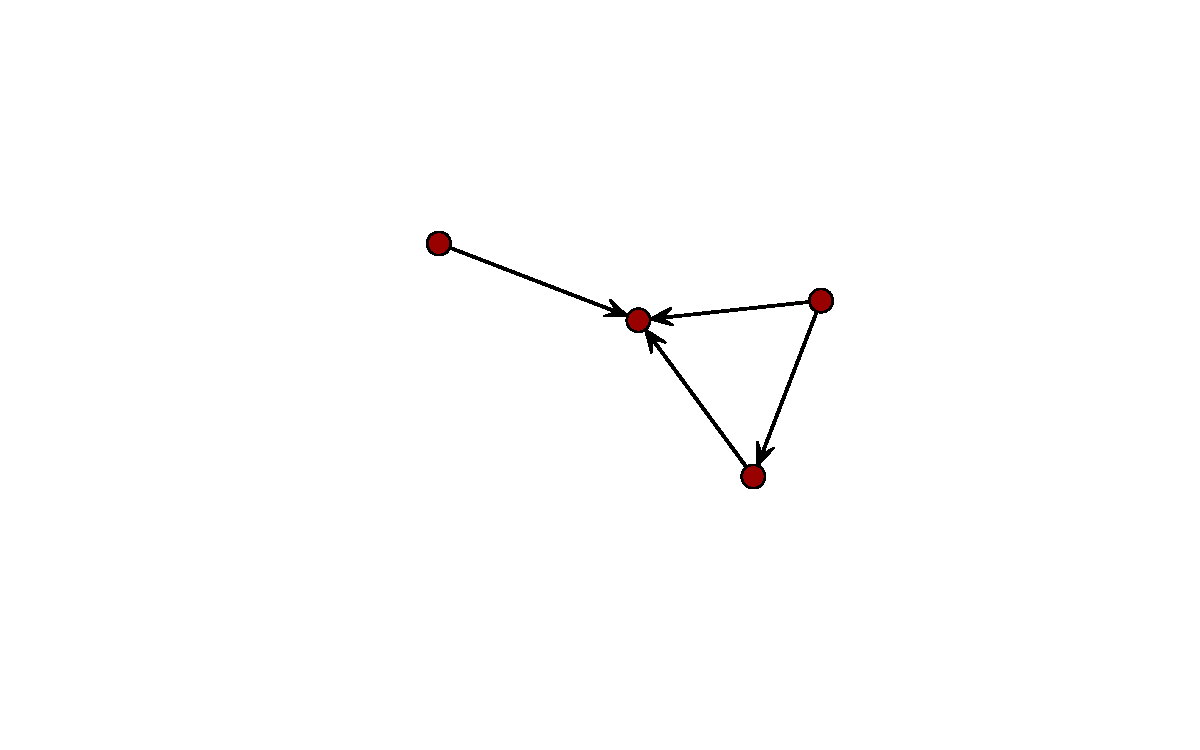
\includegraphics[width=.9\linewidth]{figure/simple-model-1} 

}



\end{knitrout}

\pause

We see 4 \textbf{edges}, 1 \textbf{transitive triad} and \textbf{no mutual ties}.

\end{column}

\pause

\begin{column}[c]{.4\linewidth}

The probability function of this model would be

\footnotesize

\begin{equation*}
\Prcond{\Graph = \graph}{\theta} = \frac{\exp{4\theta_{edges} + \theta_{ttriads} \textcolor{lightgray}{+ 0\theta_{mutual}}}}{%
\sum_{\graph'\in\GRAPH} \exp{\transpose{\theta} \sufstats{\graph'}}}
\end{equation*}

\normalsize

\noindent with $\theta = \transpose{[\theta_{edges}\quad \theta_{ttriads} \quad \theta_{mutual}]}$

\end{column}

\end{columns}



\pause

\vspace{1cm}

This model has \textbf{MLE parameter estimates} of -0.20 (low density), 0.28 (high chance of ttriads), and -Inf (low chance of mutuality) for the parameters \texttt{edges}, \texttt{ttriads}, and \texttt{mutual} respectively.

\end{frame}

% ------------------------------------------------------------------------------
\begin{frame}[label=art]
\frametitle{ERGMs: State of the Art}
\pause
Medium-large (dozens to a couple of thousand vertices) networks

\begin{itemize}
\item Markov Chain Monte Carlo (MCMC) based approaches like MC-MLE or Robbins-Monro Stochastic Approximation. \hyperlink{mcmle}{\beamergotobutton{details}}
\item Maximum Pseudo Likelihood (MPLE)
\end{itemize}\pause

large-huge networks (up to millions of vertices)

\begin{itemize}
\item Parametric bootstrap
\item Conditional joint estimation (like snowball sampling, a.k.a. divide and conquer)
\item Equilibrium Expectation Algorithm (millions of vertices)
\end{itemize}\pause

All of these methods are approximations!

\end{frame}

% ------------------------------------------------------------------------------
\begin{frame}[c]
\frametitle{Do we care about small networks?}

\begin{minipage}{.40\linewidth}
We see small networks everywhere\pause

\begin{itemize}[<+->]
\item Families and friends
\item Small teams
\item Egocentric networks
\item Online networks (sometimes)
\item etc.
\end{itemize}
\end{minipage}
\hfill
\uncover<7->{
\begin{minipage}{.55\linewidth}
\centering\large
Small networks come in samples
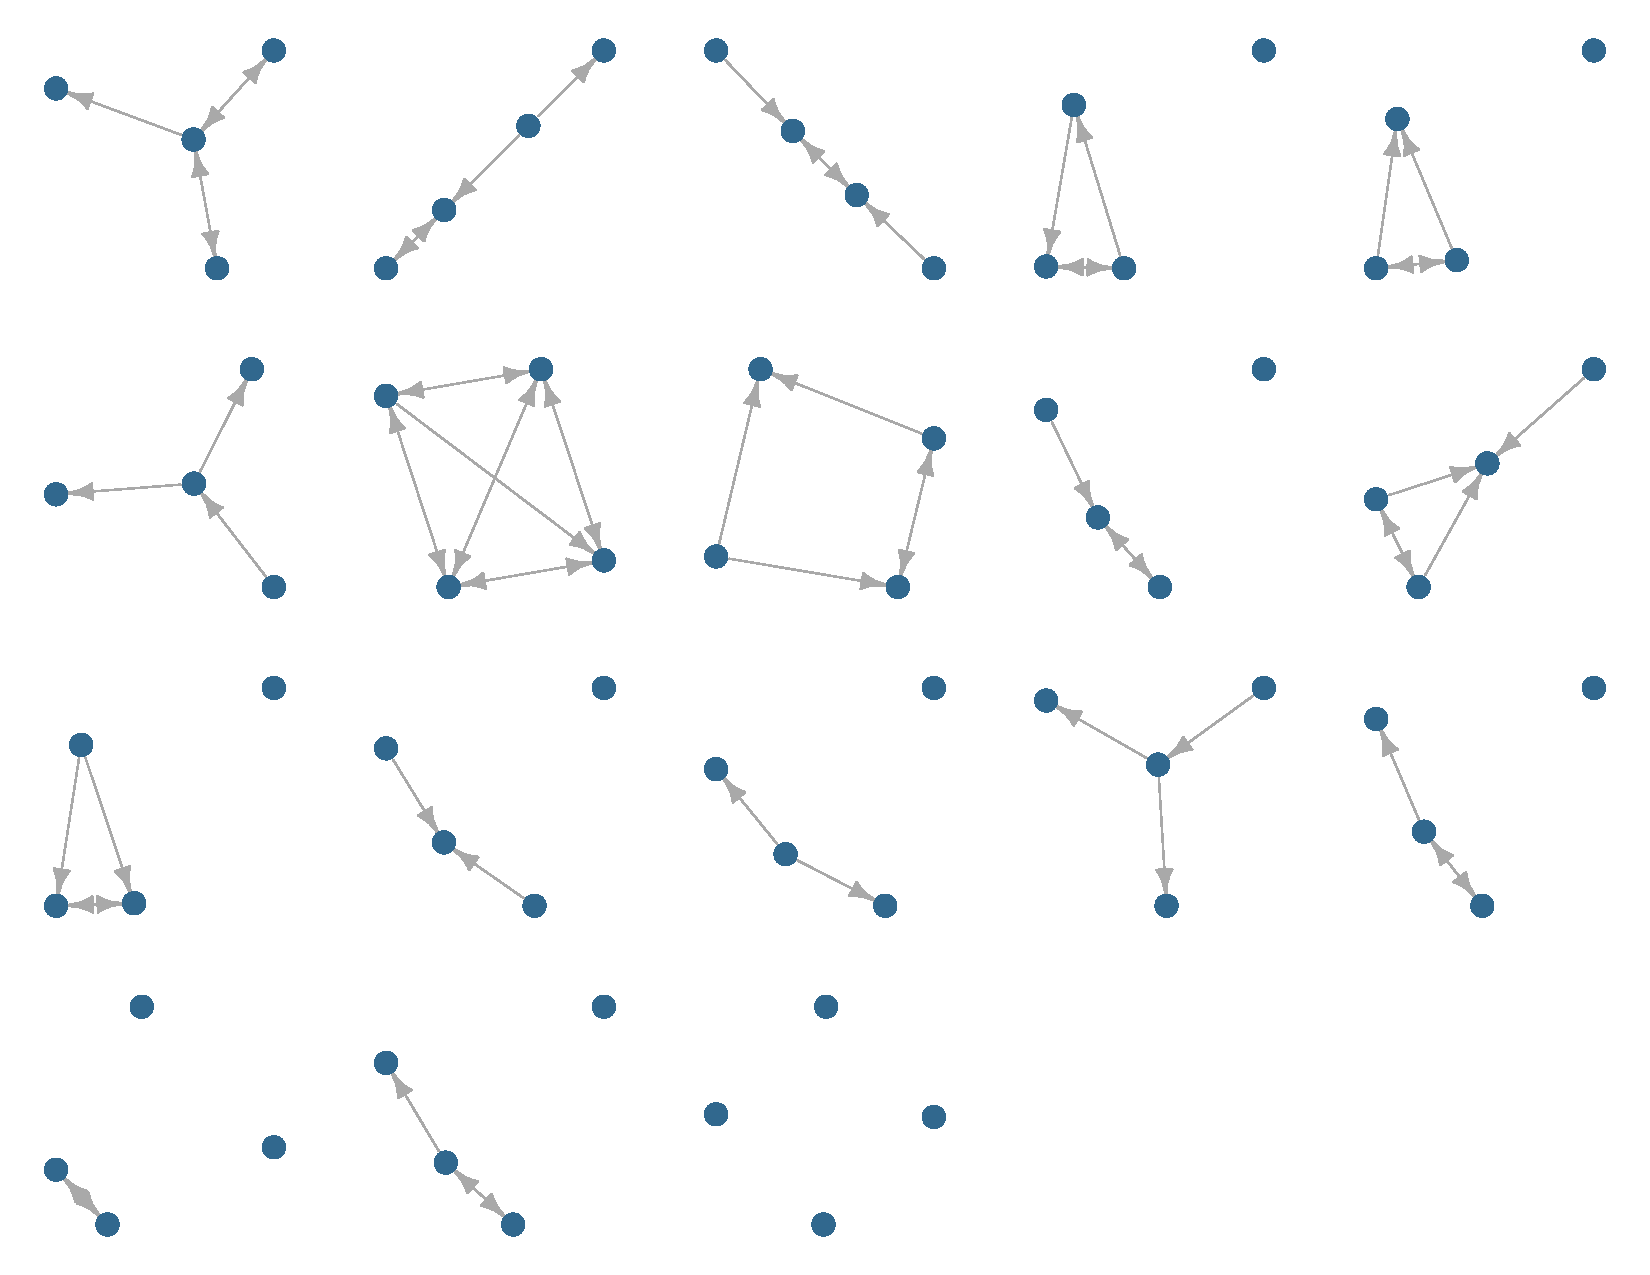
\includegraphics[width=.85\linewidth]{plot-graph-4-1.pdf}
% 
\includegraphics[width=.95\linewidth]{american-chopper-argument-ergmitos.png}
\end{minipage}
}
\end{frame}

% % ------------------------------------------------------------------------------
% \begin{frame}
% \frametitle{ERGMs for Small Networks}
% 
% From the methodological point of view, current methods are great, but:\pause
% 
% \begin{itemize}
% \item Possible accuracy issues (error rates)\pause
% \item Prone to degeneracy problems (sampling and existence of MLE)\pause
% \item It is not MLE...
% \end{itemize}
% 
% \end{frame}

% ------------------------------------------------------------------------------
\begin{frame}[label=ergmito]
\frametitle{ERGMs for Small Networks}

\uncover<3->{
\begin{figure}
\centering
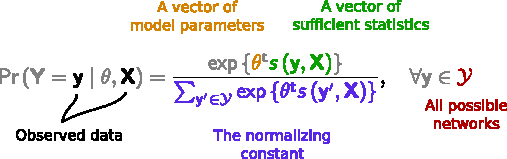
\includegraphics[width=.5\linewidth]{parts-of-ergm.pdf}
\end{figure}
}

\begin{itemize}[<+->]

\item In the case of small-enough networks, computation of the likelihood becomes
computationally feasible.

\item This allow us to directly compute {\bf\color{normconst} the normalizing constant}.\pause

\item Using the exact likelihood opens a huge window of methodological-possibilities.

\item We implemented this and more in the \ergmitopkg{} R package % \hyperlink{ergmitopkg}{\beamergotobutton{more}}
\end{itemize}


\end{frame}


% ------------------------------------------------------------------------------

\begin{frame}
Sidetrack...\vspace{.5cm}

\begin{minipage}[c]{1\linewidth}
\large \textbf{ito, ita}: From the latin -\textit{\=ittus}. suffix in Spanish used to denote small or affection. e.g.:

\hspace{.5cm} \textit{¡Qué lindo ese perr\textcolor{USCCardinal}{\textbf{ito}}!} / \textit{What a beautiful little dog!}

\hspace{.5cm} \textit{¿Me darías una tac\textcolor{USCCardinal}{\textbf{ita}} de azúcar?} / \textit{Would you give me a small cup of sugar?}
\normalsize
\end{minipage}\pause

% Screen shot of ERGMito tweet.
\vfill

\alert{Special thanks to George Barnett who proposed the name during the 2018 NASN!}

\end{frame}

% ------------------------------------------------------------------------------
\begin{frame}[label=ergmitopkg]
\frametitle{The \ergmitopkg{}}

In general

\begin{itemize}
\item Implements estimation of ERGMs using exact statistics for small networks.
\item Meta-programming allows specifying likelihood (and gradient) functions for
pooled models.% (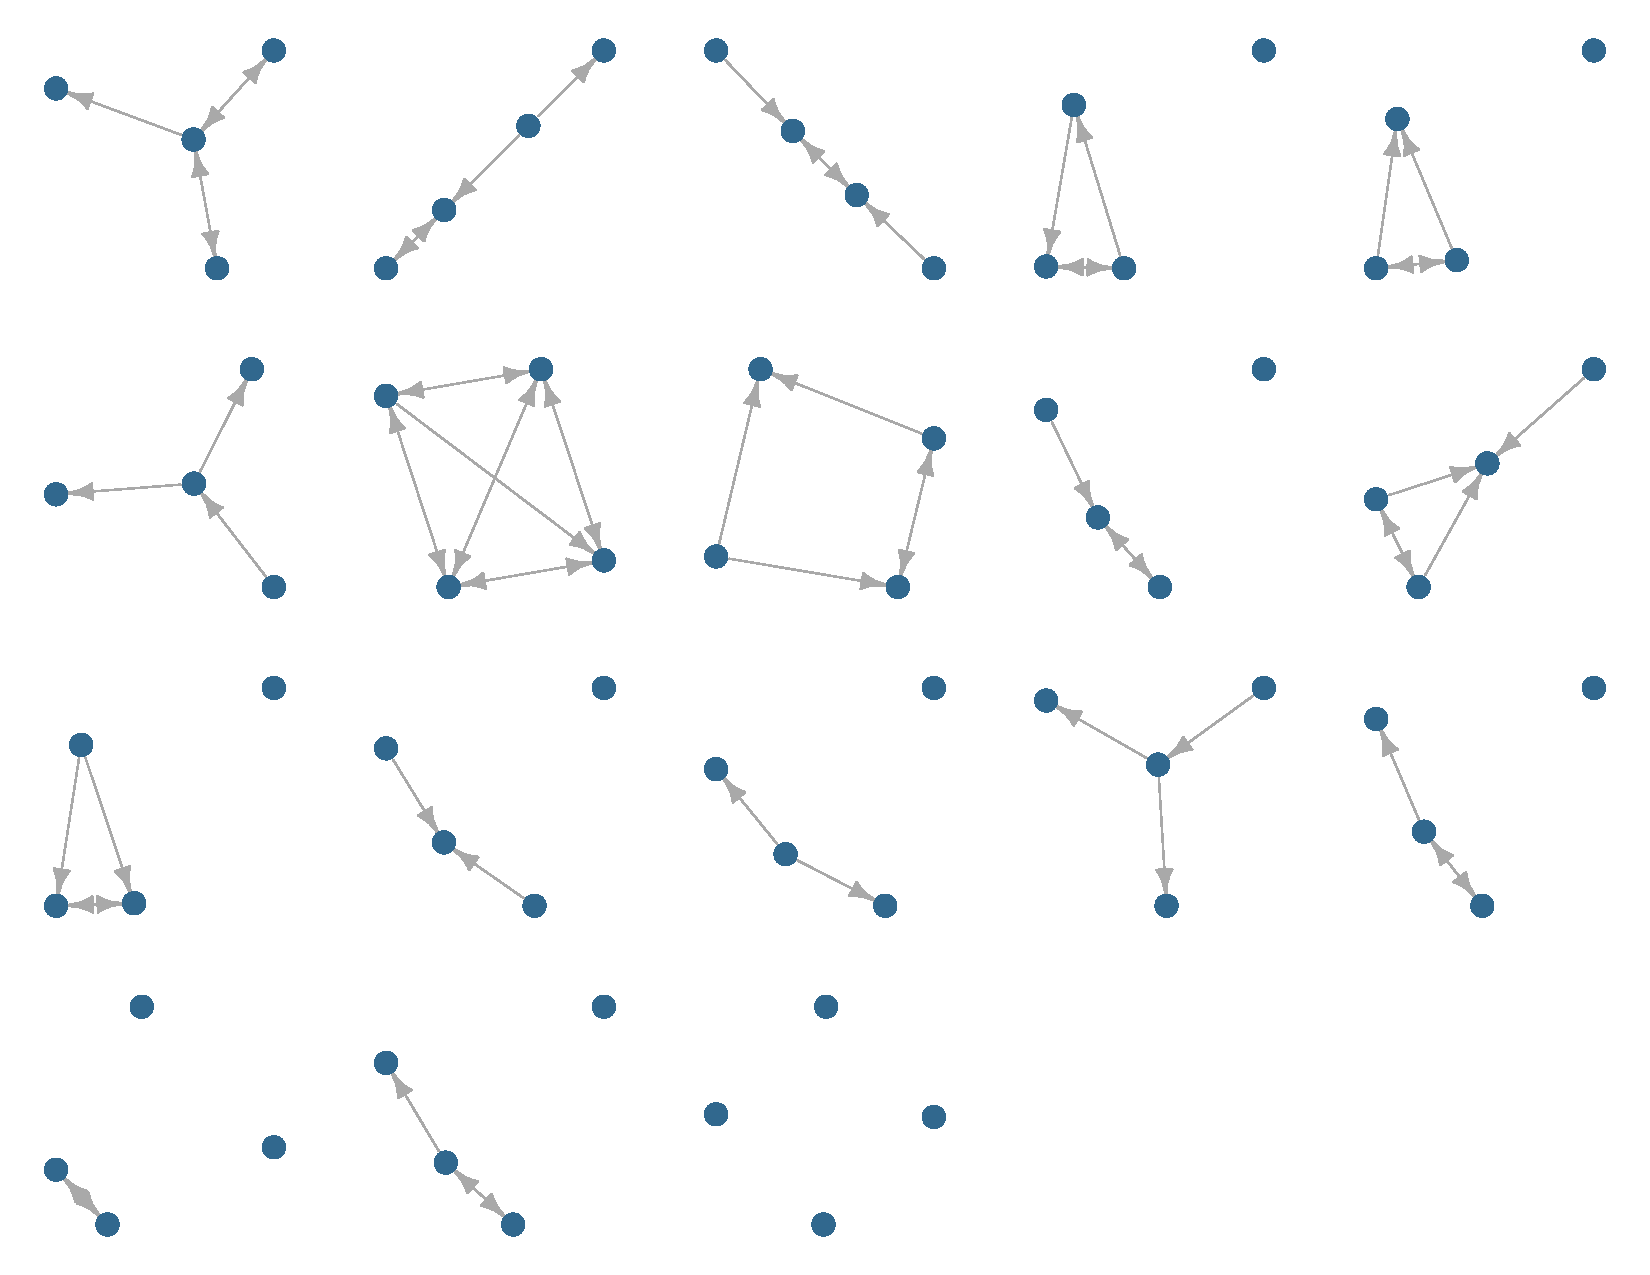
\includegraphics[width=.05\linewidth]{plot-graph-4-1.pdf}).
\item Includes tools for simulating and post-estimation checks.
\item Getting ready for CRAN!
\end{itemize}\pause

Other features

\begin{itemize}
% \item Computes support of Pr using \texttt{ergm::ergm.allstats}
\item Vectorized calculation of sufficient statistics.
\item Scales up nicely (hundreds of small networks) saving space and computation (when possible).
\item Highly tested (90\% coverage with more than one hundred tests).
\end{itemize}

% \vfill\hfill \hyperlink{ergmito}{\beamerreturnbutton{go back}}

\end{frame}

% ------------------------------------------------------------------------------
\begin{frame}[label = ergmitoexample]
\frametitle{\ergmitopkg{} example}

\begin{minipage}{.4\linewidth}
\begin{figure}
\centering
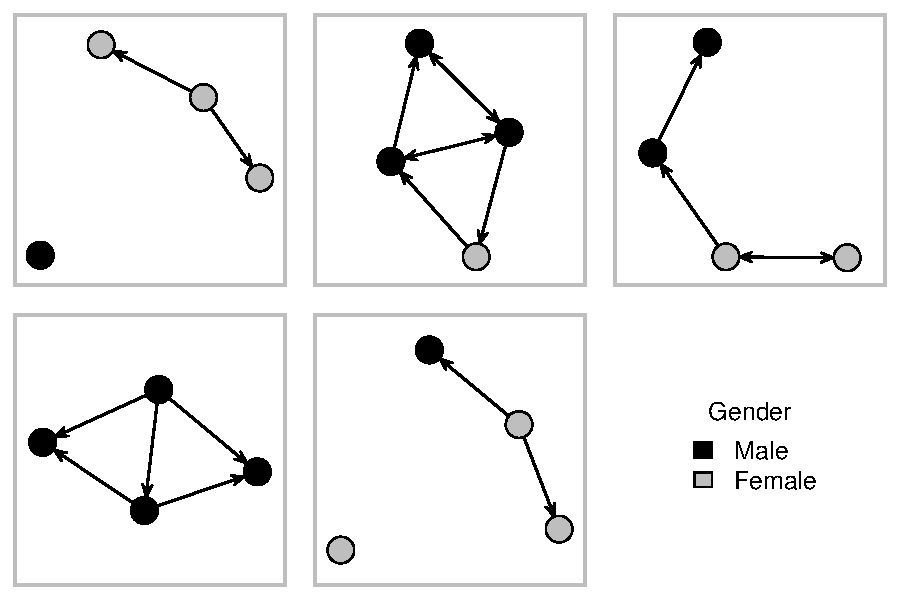
\includegraphics[width = .9\linewidth]{fivenets_graphs.pdf}
\caption{Random sample of 5 networks simulated using the ergmito package}
\end{figure}
\end{minipage}
\hfill
\begin{minipage}{.55\linewidth}
\pause
\footnotesize
\begin{table}
\begin{tabular}{l*{2}{m{.2\linewidth}<\centering}}
\hline
 & Bernoulli & Full model \\
\hline
Edge-count             & $-0.69^{*}$ & $-1.70^{**}$ \\
                      & $(0.27)$    & $(0.54)$     \\
Homophily (on Gender) & & $1.59^{*}$   \\
                      & & $(0.64)$     \\
\hline
AIC                   & 78.38       & 73.34        \\
BIC                   & 80.48       & 77.53        \\
Log Likelihood        & -38.19      & -34.67       \\
Num. networks         & 5           & 5            \\
\hline
\multicolumn{3}{l}{\scriptsize{Standard errors in parenthesis. $^{***}p<0.001$, $^{**}p<0.01$, $^*p<0.05$}}
\end{tabular}
\caption{Fitted ERGMitos using the fivenets dataset.}
\label{table:coefficients}
\end{table}
\normalsize
\end{minipage}\pause

We performed a large simulation study \hyperlink{ergmitodgp}{\beamergotobutton{more}}
comparing MC-MLE (ergm) with MLE (ergmito).

\end{frame}

% ------------------------------------------------------------------------------
\begin{frame}[label=ergmsims,allowframebreaks]
\frametitle{Paper 2 Simulation Studies: Error rate}

\begin{minipage}{.45\linewidth}
\begin{itemize}[<+->]
\item The MC-MLE implementation failed $\sim$ 5,000/20,000 times
\item In $\sim$700 of those cases ergmito (MLE) reported a significant effect
\item I no case that MLE failed MC-MLE reported an effect.
\end{itemize}
\end{minipage}
\hfill
\begin{minipage}{.45\linewidth}
\begin{figure}
\centering
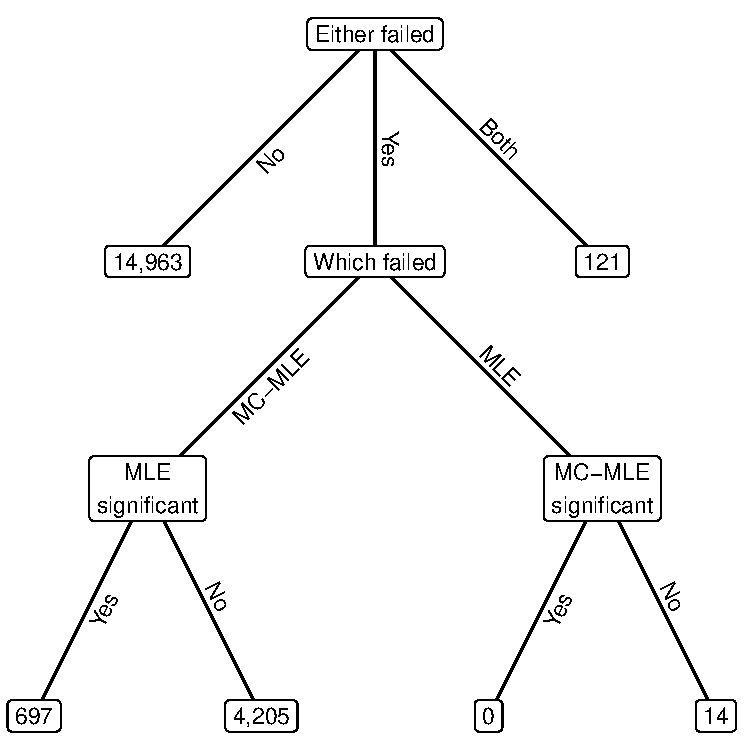
\includegraphics[width=.9\linewidth]{failed-tree.pdf}
\end{figure}
\end{minipage}

% \hyperlink{ergmitoexperiment}{\beamerreturnbutton{go back}}

\end{frame}

% ------------------------------------------------------------------------------
\begin{frame}
\frametitle{Paper 2 Simulation Studies: Empirical Type I error}

\footnotesize

\begin{table}[ht]
	\centering
	\begin{tabular}{cccc}
		\toprule & \multicolumn{2}{c}{P(Type I error)} \\ \cmidrule(r){2-3}
		Sample size  & \makecell{MC-MLE \\ (\ergmpkg{})} & \makecell{MLE \\ (\ergmitopkg{})} & $\chi^2$ \\ 
		\midrule
		5 & 0.084 & 0.057 & 11.71 *** \\ 
		10 & 0.070 & 0.045 & 12.46 *** \\ 
		15 & 0.084 & 0.066 & 5.55 * \\ 
		20 & 0.074 & 0.060 & 3.58  \\ 
		30 & 0.057 & 0.052 & 0.67  \\ 
		50 & 0.046 & 0.044 & 0.17  \\ 
		100 & 0.048 & 0.048 & 0.00  \\ 
		\bottomrule
	\end{tabular}
	\caption{\label{tab:typeI}Empirical Type I error rates. The $\chi^2$ statistic is from a 2-sample test for equality of proportions, and the significance levels are given by *** $p < 0.001$, ** $p < 0.01$, and * $p < 0.05$.} 
\end{table}

\end{frame}

% ------------------------------------------------------------------------------
\begin{frame}[label=ergmitoexperiment]
\frametitle{Paper 2 Simulation Studies: Elapsed time}

\begin{figure}
\centering
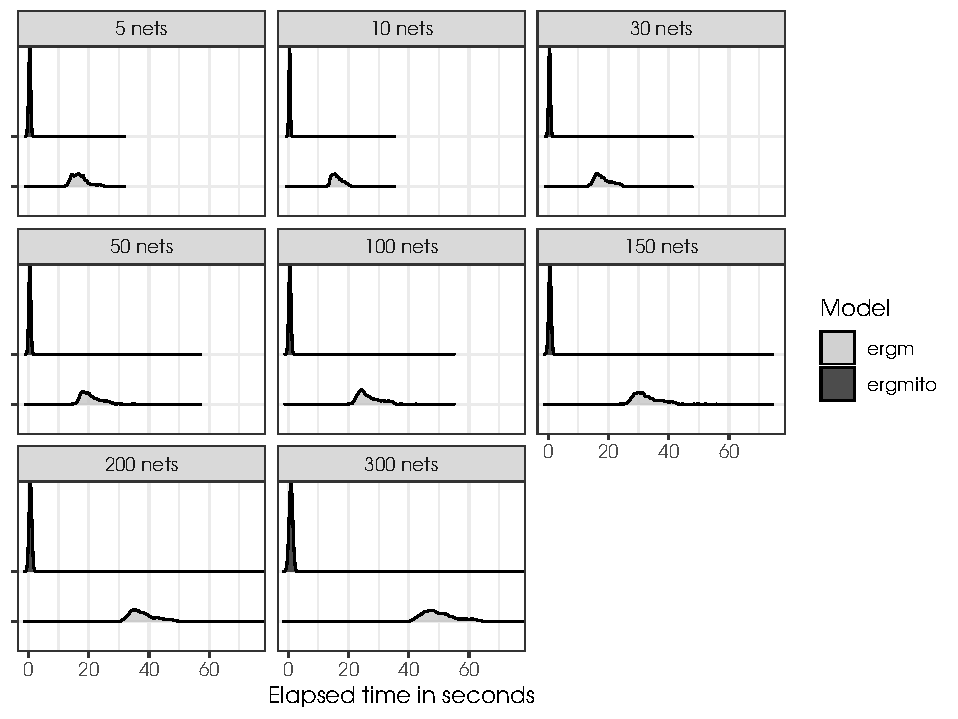
\includegraphics[width=.6\linewidth]{bias-elapsed-02-various-sizes-4-5-ttriad.pdf}
\end{figure}

\vfill\hfill\hyperlink{ergmito-bias}{\beamergotobutton{more results}}

\end{frame}

% ------------------------------------------------------------------------------
\begin{frame}
\frametitle{Paper 2: Exponential Random Graph Models for Small Networks}

{\bf \large Key takeaways}\pause
\setbeamercolor{conclusions}{bg=usclightgray!60!white, fg=uscdarkgray}
\begin{beamercolorbox}[dp=1ex]{conclusions}
\begin{itemize}
\item New extension of ERGMs using exact statistics for small networks
(families, teams, etc.)\pause
\item Performance: Same (un)bias, Lower Type I error rates, (way) faster.\pause
\item Opens the door the new methods, e.g. Mixed effects, LRT, etc.
\end{itemize}
\end{beamercolorbox}

\vfill\pause

{\bf \large Challenges}
\begin{beamercolorbox}[dp=1ex]{conclusions}
\begin{itemize}
\item Computationally, we can do better in terms of speed/memory.\pause
\item Have a good way of assessing goodness-of-fit.\pause
\item Explore extending this method for (very) large networks.
\end{itemize}
\end{beamercolorbox}

\end{frame}

% ------------------------------------------------------------------------------
% ------------------------------------------------------------------------------
% ------------------------------------------------------------------------------
% ------------------------------------------------------------------------------
\section{Future Research}

\begin{frame}[c]
\usebeamertemplate{section intro}{}{}
\textcolor{uscgold}{
\Large {\bf Future Research}
}
\end{frame}

% ------------------------------------------------------------------------------
\begin{frame}[t]
\frametitle{Future Research: ERGMitos}

{\bf Goodness-of-fit}\pause
\begin{itemize}
\item Is something that will need to be addressed at some point.\pause
\item The problem is not easy as we need to deal a discrete distribution.\pause
\item Two key questions: What sufficient statistic to look at? what test?
\end{itemize}

\pause {\bf ERGMs for large networks} \pause
\begin{itemize}
\item There is still no standard way to estimate ERGMs for large networks.\pause
\item Most attempts are still depending on simulation methods.\pause
\item We could use the Snowball Sampling framework together with ERGMitos.\pause{}
(... I would call this ERGMote)
\end{itemize}

\end{frame}

% % ------------------------------------------------------------------------------
\begin{frame}[t]
\frametitle{Concluding Remarks}

% \large {\bf Accomplished so far}
\begin{itemize}[<+->]
  \item An extension to a well studied models for social networks.
  \item Small size allows exact calculations.
  \item Opens the door to a large set of methodological innovations.
  \item \textbf{Next steps:} GOF or extensions to large networks?
\end{itemize}

\vfill
\footnotesize 
\uncover<5->{{\bf Accomplishments during the development of this work}
\begin{beamercolorbox}{conclusions}
\begin{itemize}
\item 6 journal publications (Journal of Open Source Software, Stata Journal, Journal of health and social behavior, Translational behavioral medicine, Social Science \& Medicine)
\item 11 packages/libraries built (ergmito, similR, gnet, fmcmc, slurmR, aphylo, polygons, pruner, netplot, rphyloxml, jsPhyloSVG)
\end{itemize}
\end{beamercolorbox}
}
\end{frame}

% % ------------------------------------------------------------------------------
\begin{frame}
\maketitle
\begin{center}
\scalebox{2}{\textcolor{uscgold}{Thanks!}}
\end{center}
\end{frame}

\renewcommand{\section}[2]{}%
\appendix
\begin{frame}[allowframebreaks]
\frametitle{References}
% \bibliographystyle{apacite}
% \bibliography{bibliography.bib}
\printbibliography
\end{frame}


% ------------------------------------------------------------------------------
% ------------------------------------------------------------------------------
% ------------------------------------------------------------------------------
% ------------------------------------------------------------------------------
% ------------------------------------------------------------------------------


% ------------------------------------------------------------------------------
\begin{frame}[label=mcmle]
\frametitle{ERGMs: The MC-MLE approach}

One of the most popular methods for estimating ERGMs is the MC-MLE approach (citations here)

This consists on the following steps

\begin{enumerate}
\item Start from a sensible guess on what should be the population parameters
(usually done using pseudo-MLE estimation)
\item While the algorithm doesn't converge, do:
  \begin{enumerate}
  \item Simulate a stream of networks with the current state of the parameter,
  $\theta_t$
  \item Using the law of large numbers, approximate the ratio of likelihoods 
  based on the parameter $\theta_t$, this is the objective function
  \item Update the parameter by a Newton-Raphson step
  \item Next iteration
  \end{enumerate}
\end{enumerate}

\vfill\hfill \hyperlink{art}{\beamerreturnbutton{go back}}


\end{frame}



% ------------------------------------------------------------------------------
\begin{frame}[label=ergmitodgp]
\frametitle{Paper 2 Simulation Studies}

We performed a simulation study with the following features:

\begin{itemize}%[<+->]
\item Draw 20,000 samples of groups of small networks
\item Each group had prescribed: (model parameters, number of networks, sizes of the networks)
\item Each group could have from 5 to 300 small networks
\item We estimated the models using MC-MLE and MLE.
\end{itemize}

\vfill\hfill\hyperlink{ergmitoexample}{\beamerreturnbutton{go back}}

\end{frame}



% ------------------------------------------------------------------------------
\begin{frame}[label=ergmito-bias]
\frametitle{Paper 2 Simulation Studies: Empirical Bias}

\begin{figure}
\centering
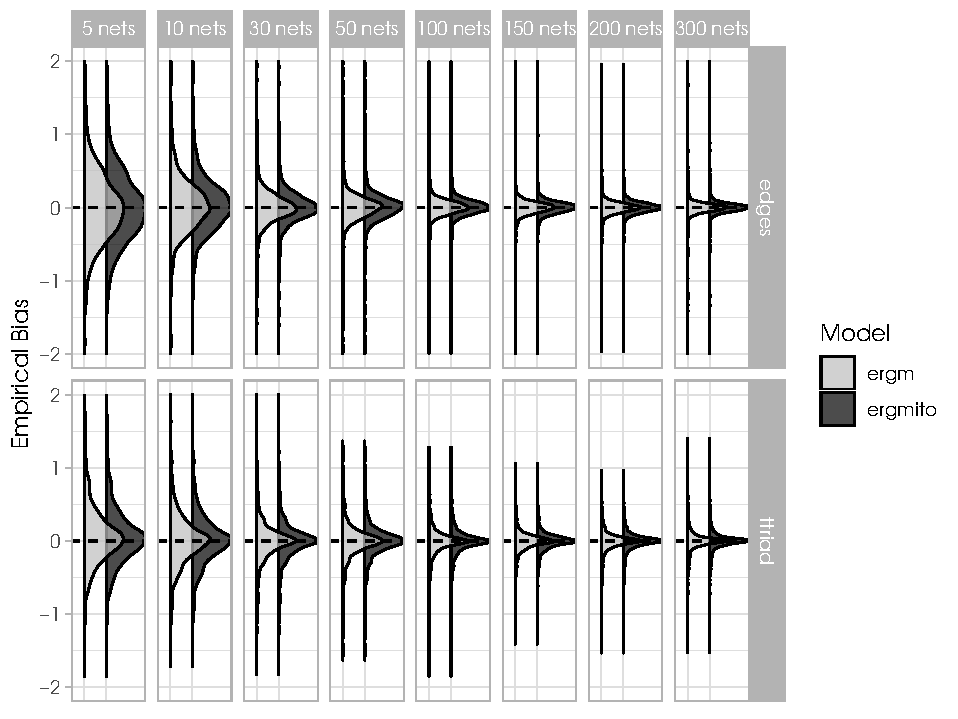
\includegraphics[width=.6\linewidth]{bias-02-various-sizes-4-5-ttriad.pdf}
\end{figure}

\vfill\hfill \hyperlink{ergmitoexperiment}{\beamerreturnbutton{go back}}

\end{frame}

\end{document}

